\section{Combining MRST and Gmsh}
\label{sec:combining}
As MRST and Gmsh both have their limitations, adopting Gmsh into an MRST workflow may be beneficial. This section will discuss an existing method for loading Gmsh meshes, \nameref{sec:GmshToMRST}, and introduce a new package for integrating the two, \nameref{sec:own_software}.

\subsection{\texttt{gmshToMrst}}
\label{sec:GmshToMRST}
Originally developed by \textcite{gmsh_to_mrst} as a stand-alone method for loading Gmsh meshes into MRST, \verb|gmshToMrst| became part of MRST's module library with release \verb|2022a|. The module reads the mesh from an \verb|.m|-file and performs the necessary computations for converting the mesh to an MRST grid. While it does this job well, one key requirement of \verb|gmshToMrst| is that the Gmsh mesh has been computed beforehand. This requires users to manually create the Gmsh mesh, slowing down the rapid prototyping MRST is designed to perform, while forcing its users to learn an entirely new program in order to generate the grids.

% \verb|gmshToMRST| is a MATLAB module for loading created Gmsh meshes. 

\subsection{\texttt{gmsh4mrst}}
\label{sec:own_software}
To help with this, I have developed a new software module, \verb|gmsh4mrst|, to enable automatic Gmsh mesh generation from MATLAB. By abstracting most of the manual work required for generating meshes in Gmsh, \verb|gmsh4mrst| is designed to enable users to use Gmsh as a backend for mesh creation, speeding up the mesh generation of detailed domains, without the user having to spend time learning a new software. The goal of \verb|gmsh4mrst| is to enable a near drop-in replacement of \verb|distmesh| with Gmsh-created meshes.


\subsubsection{Installation}
In order to integrate the two systems, \verb|gmsh4mrst| is split in two parts, one written in Python and one in MATLAB. The Python package is hosted on PyPi \cite{gmsh4mrst}, and can easily be installed from there. The MATLAB package must be manually downloaded, and the files must be added to the MATLAB path.

The Python package works as a stand-alone package. The MATLAB package, however, uses Python to create base meshes, and therefore requires that the Python package is installed to run. MATLAB must be run from an environment with the Python package installed, whether that is through a virtual environment or the base Python installation on the computer.


\subsubsection{Features}
The primary target of \verb|gmsh4mrst| is to automate Gmsh mesh creation for use in MRST grids, while maintaining the flexibility needed for optimal grid creation. Care has been taken to ensure \verb|gmsh4mrst| is as robust as possible, especially when it comes to connecting MATLAB and Python.

One key feature of \verb|gmsh4mrst| is its many user-settable arguments and parameters. By leaving most grid-refinement decisions to the user, \verb|gmsh4mrst| can be used for almost every grid creation necessary, while reasonable defaults ensure the module can be used for simple grids without much time spent on refinement. The module easily handles complex, non-convex domains, and is designed to adapt the grid to all face- and cell constraints.

\subsubsection{Python package}
The Python part of \verb|gmsh4mrst| is where most of the grid generation is done. While the actual implementation and specifications may change over time, the Python package currently implements three methods.

\paragraph{\texttt{background\_grid\_2D}:}
The most basic of the implemented methods, \verb|background_grid_2D| uses Gmsh to create a simple background triangulation without any embedded points or lines, but with refinement around face- and cell constraints. This results in a uniform mesh, and can be used as a straight replacement of the Distmesh algorithm. The user has detailed control of the mesh, including any refinement done along the constraints.

\paragraph{\texttt{delaunay\_grid\_2D}:}
Going one step further, \verb|delaunay_grid_2D| creates a background triangulation, but include the constraints in the generated mesh. Face constraints are embedded directly as lines or points, ensuring that the faces of the resulting Delaunay triangulation align with the constraints. Each cell constraint is wrapped in a transfinite mesh, ensuring the constraints are traced with cells in the triangulation. As a result of using transfinite meshes, \verb|delaunay_grid_2D| fails if any cell constraints intersect either each other or any face constraints.

\paragraph{\texttt{pebi\_base\_2D}:}
The most complex of the implemented methods, \verb|pebi_base_2D| creates a background triangulation, but include both face- and cell constraints as transfinite meshes. The idea behind this is that it ensures a distribution of Delaunay vertices -- and by extension PEBI sites after converting the triangulation -- around the constraints, ensuring face constraints are traced by PEBI faces and cell constraints by PEBI sites. As a result of using transfinite meshes, \verb|pebi_base_2D| fails if any constraints intersect.

All methods implemented in the Python package output Delaunay triangulations. The difference in outputs of the methods is shown in \autoref{fig:gmsh4mrst-pymethods}, where the left sides of the grids contain face constraints, and the right sides contain cell constraints.

\begin{figure}[p]
    \centering
    \begin{subfigure}[b]{0.49\textwidth}
        \centering
        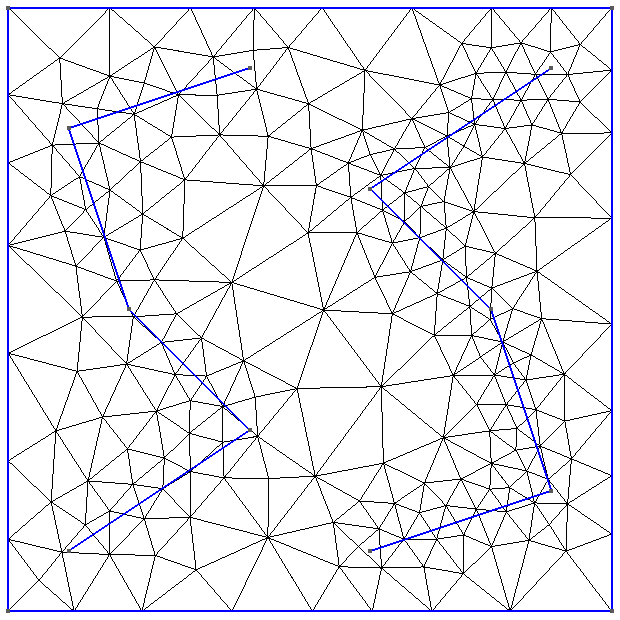
\includegraphics[width=\textwidth]{report/Images/Combining software/Demo gmsh4mrst/demo_background_grid_2D_lines.png}
        \caption{\texttt{background\_grid\_2D}}
        \label{fig:background_grid_2D}
    \end{subfigure}
    \begin{subfigure}[b]{0.49\textwidth}
        \centering
        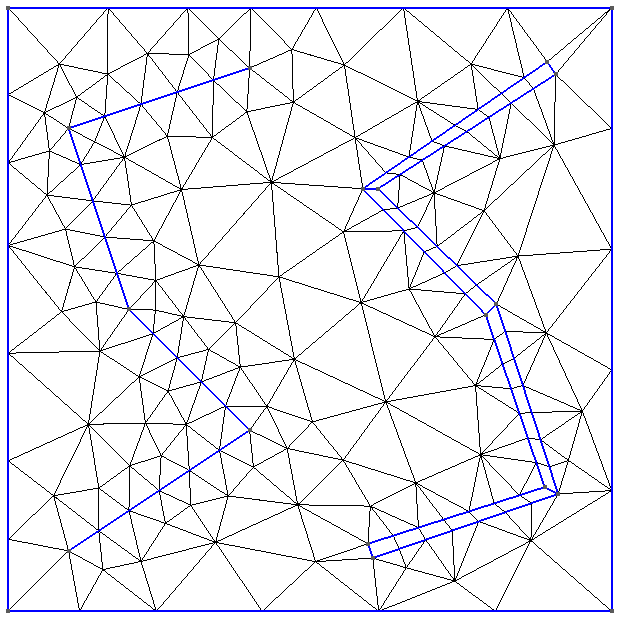
\includegraphics[width=\textwidth]{report/Images/Combining software/Demo gmsh4mrst/demo_delaunay_grid_2D_lines.png}
        \caption{\texttt{delaunay\_grid\_2D}}
        \label{fig:delaunay_grid_2D}
    \end{subfigure}
    \begin{subfigure}[b]{0.49\textwidth}
        \centering
        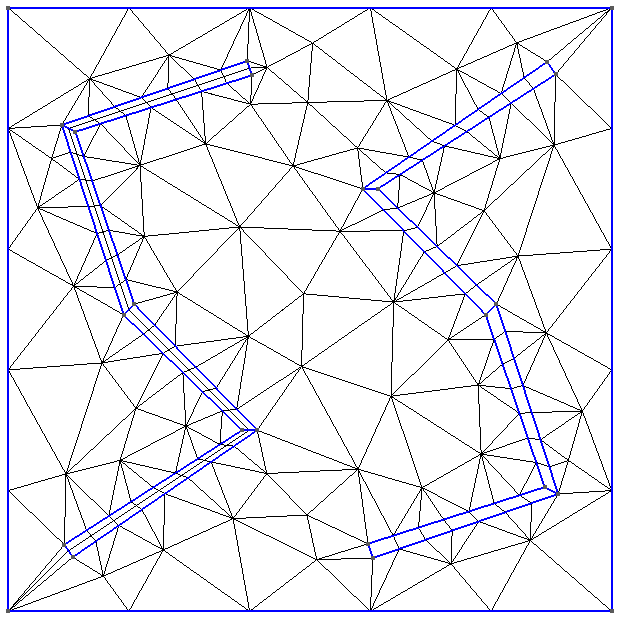
\includegraphics[width=\textwidth]{report/Images/Combining software/Demo gmsh4mrst/demo_pebi_base_2D_lines.png}
        \caption{\texttt{pebi\_base\_2D}}
        \label{fig:pebi_base_2D}
    \end{subfigure}
    \caption{Comparison of the Python methods implemented in \texttt{gmsh4mrst}.}
    \label{fig:gmsh4mrst-pymethods}
\end{figure}

\subsubsection{MATLAB package}
The MATLAB part of \verb|gmsh4mrst| contains all code for converting the Gmsh meshes to MRST grids, as well as some code for creating PEBI sites. While the actual implementation and specifications may change over time, the MATLAB package currently implements three methods. 

\paragraph{\texttt{pebiGrid2DGmsh}:}
Designed to be a semi-direct replacement of MRST's \verb|pebiGrid2D|, \verb|pebiGrid2DGmsh| uses \verb|background_grid_2D| to create a background grid, then creates well and fracture sites in MATLAB. This gives it the same flexibility and robustness as \verb|pebiGrid2D|, while avoiding the slow site distribution of Distmesh. The method works nicely for face constraints, but struggles somewhat with aligning cell constraints accurately.

\paragraph{\texttt{delaunayGrid2DGmsh}:}
The most direct of the MATLAB methods, \verb|delaunayGrid2DGmsh| uses \verb|delaunay_grid_2D| to create a Delaunay triangulation capturing the supplied constraints, then converts it to an MRST grid directly. As no conversion is done, this leaves the output grid as a Delaunay triangulation, but it avoids the extra work of converting without losing constraint information. Due to using \verb|delaunay_grid_2D|, no cell constraints may intersect.

\paragraph{\texttt{pebiGrid2DGmshBase}:}
As a somewhat experimental method, \verb|pebiGrid2DGmshBase| uses \verb|pebi_base_2D| to create a triangulation with constraints embedded as transfinite meshes. The user can then choose whether to convert the triangulation to a PEBI grid or not. This results in a relatively flexible method, but due to using \verb|pebi_base_2D|, no constraints may intersect.

All the MATLAB methods gives the user complete control of all parameters of the underlying Python grid creation, with \verb|pebiGrid2DGmsh| additionally letting the user control the fault- and well site creation done in MATLAB. The difference in outputs of the methods is shown in \autoref{fig:gmsh4mrst-MATLABmethods}, where the left sides of the grids contain face constraints, and the right sides contain cell constraints.

\begin{figure}[p]
    \centering
    \begin{subfigure}[b]{0.49\textwidth}
        \centering
        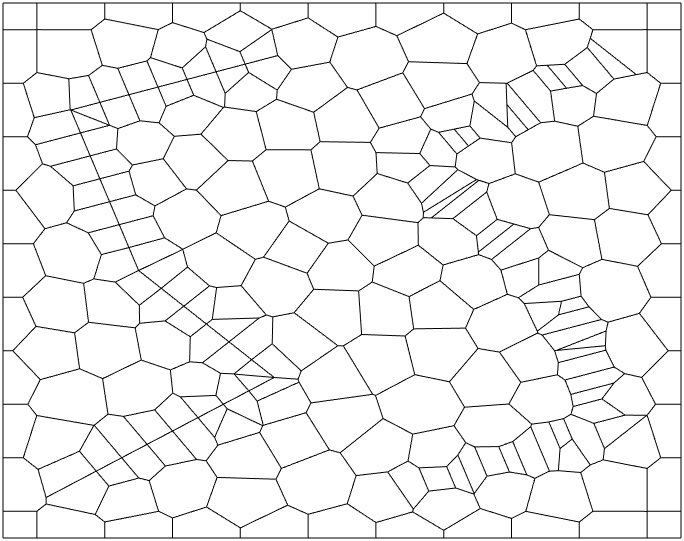
\includegraphics[width=\textwidth]{report/Images/Combining software/Demo gmsh4mrst MATLAB/demo_pebiGrid2DGmsh.png}
        \caption{\texttt{pebiGrid2DGmsh}}
        \label{fig:pebiGrid2DGmsh}
    \end{subfigure}
    \begin{subfigure}[b]{0.49\textwidth}
        \centering
        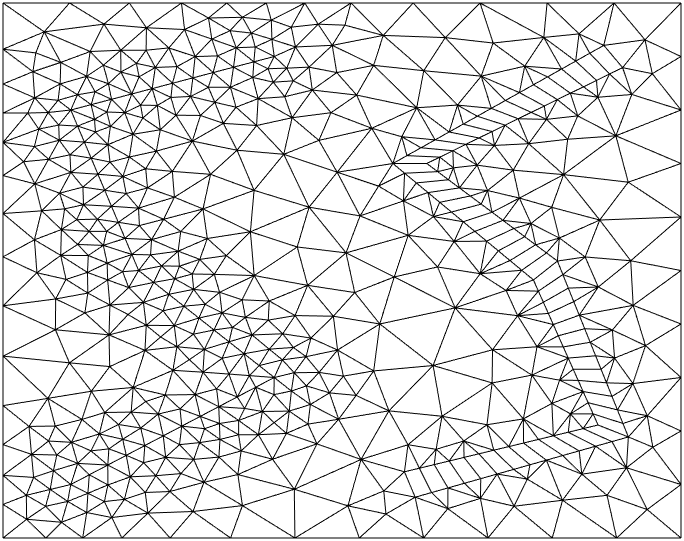
\includegraphics[width=\textwidth]{report/Images/Combining software/Demo gmsh4mrst MATLAB/demo_delaunayGrid2DGmsh.png}
        \caption{\texttt{delaunayGrid2DGmsh}}
        \label{fig:delaunayGrid2DGmsh}
    \end{subfigure}
    \begin{subfigure}[b]{0.49\textwidth}
        \centering
        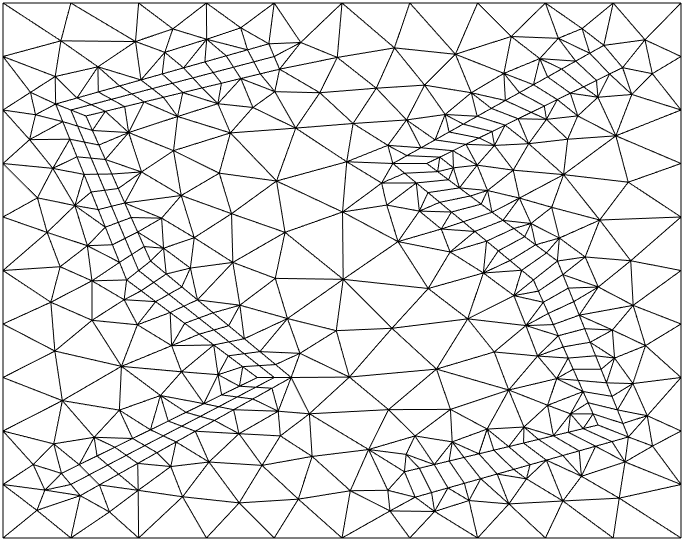
\includegraphics[width=\textwidth]{report/Images/Combining software/Demo gmsh4mrst MATLAB/demo_pebiGrid2DGmshBase.png}
        \caption{\texttt{pebiGrid2DGmshBase}}
        \label{fig:pebiGrid2DGmshBase}
    \end{subfigure}
    \begin{subfigure}[b]{0.49\textwidth}
        \centering
        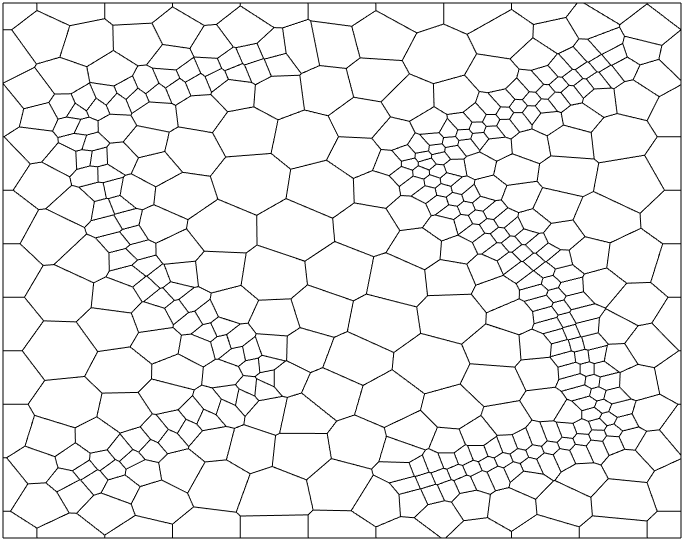
\includegraphics[width=\textwidth]{report/Images/Combining software/Demo gmsh4mrst MATLAB/demo_pebiGrid2DGmshBase_PEBI.png}
        \caption{\texttt{pebiGrid2DGmshBase} as PEBI}
        \label{fig:pebiGrid2DGmshBase_PEBI}
    \end{subfigure}
    \caption{Comparison of the MATLAB methods implemented in \texttt{gmsh4mrst}.}
    \label{fig:gmsh4mrst-MATLABmethods}
\end{figure}

\subsubsection{Arguments}
% Table of arguments
% Python  |  MATLAB  |  Explanation?  |  Default value

\subsubsection{Implementations}
% Deep-dive into the mechanics of gmsh4MRST
% How the different features are implemented, concretely
% Discuss Fields, constraint implementation (especially cell constraints), etc.
% Perhaps discuss Gmsh meshing and recombination algorithms
% Argument handling, how it handles arguments in several different formats
\paragraph{Face constraints:}
\paragraph{Cell constraints:}
\paragraph{Mesh refinement:}
\paragraph{Integrating MATLAB and Python:}

\subsubsection{Limitations}
% clippedPebiGrid2DGmsh slow for multiple cell constraints
% Fiddling required to get non-triangular grids (which is Gmsh's default)
% Highly structured cell constraints - may be cases where this is suboptimal
% Face- and cell constraints can NOT cross each other, mesh will not compile!
% Struggles somewhat with crossing face constraints - inaccurate where they overlap
% API compitability (same arguments) as UPR's pebiGrid2D
% Does not compute centroidal voronoi diagrams -> suboptimal distribution of centers?

% Likely from GmshToMRST
\begin{codeError}
Warning: No field 'faces.neighbors' found. Adding plausible values... proceed with caution! 
\end{codeError}
